\documentclass{ltjsbook}
\usepackage{docmute} 
\usepackage{../../myStyle} 

\begin{document}
% \chapter{構造方程式モデリング}
\chapter{Structural Equation Modelling}
\label{x12_SEM}

% 本項では\keyterm{構造方程式モデリング}{こうぞうほうていしきもでりんぐ}{Structural Equation Modeling, SEM}について説明していきます\footnote{この手法は別名\keytermL{共分散構造分析}{きょうぶんさんこうぞうぶんせき}という名前でも呼ばれています。書籍や論文を検索する時は，こちらの名称もキーワードにしてみてください。}。この手法はこれまで学んできた因子分析や回帰分析を統合したもので，分散共分散行列に方程式を作り込んでいくものです。我々が調査で得たデータから得られる情報は，分散共分散行列がすべてですから，その変数間関係を細かく作り込んでいき，行列の隅々まで考え尽くすという意味で，究極の手法といえるでしょう。実際，SEMは因子分析や回帰分析の他にも，多くのモデルをその下位モデルとして包含します。言い換えれば，SEMが登場する前に考えられてきたさまざまなモデルが，SEMの枠組みで理解・表現できるようになりました。であれば，この究極の技さえ知っておけば，非常に広範囲に拡張できるわけですから，こんなに便利なことはありません。
In this section, we will explain \keyterm{Structural Equation Modeling, SEM}. This method is also known as \keytermL{covariance structure analysis}, so when searching for books or papers, please try using this name as a keyword. This method integrates the factor analysis and regression analysis we have learned so far, and embeds equations into the variance-covariance matrix. Since all the information we can get from the data we collect in a survey is in the variance-covariance matrix, we can say that it is the ultimate method in the sense that it finely constructs the relationship between variables and thinks through to every corner of the matrix. In fact, in addition to factor analysis and regression analysis, SEM includes many other models as its sub-models. In other words, various models that were thought of before the advent of SEM can now be understood and expressed within the framework of SEM. Therefore, if you know this ultimate technique, you can extend it to a very wide range, which is extremely convenient.

% このように技術的には非常に高度なものでありますが，これを使うのは意外と簡単にできます。モデルをイメージで表現できる，パスダイアグラムの考え方から入っていきましょう。
Although this is technically very advanced, it is surprisingly easy to use. Let's start with the concept of a path diagram, which allows us to represent the model visually.

% \section{パスダイアグラムの書き方}
\section{How to Write a Path Diagram}
% 変数間の関係を表す図を\keytermL{パス図}{ぱすず}あるいは\keyterm{パスダイアグラム}{ぱすだいあぐらむ}{Path Diagram}と言います。
The diagram that represents the relationship between variables is called a "Path Diagram" or "Path Diagram".

% 分析する際の変数には\keyterm{観測変数}{かんそくへんすう}{Observed Variables}と\keyterm{潜在変数}{せんざいへんすう}{Latent Variables}があります。観測変数はその名の通り，観測された変数であり，データとして数値化されたものになります。これに対して潜在変数とは，モデルで仮定された変数のことです。たとえば因子分析やテスト理論では，因子や学力といったものを想定します。それが潜在変数です。潜在変数はデータとして数値化されているのではなく，抽象的な概念ですが，図にする場合はそれも表現しなければなりません。
During analysis, there are variables called \keyterm{Observed Variables}{かんそくへんすう}{Observed Variables} and \keyterm{Latent Variables}{せんざいへんすう}{Latent Variables}. As the name suggests, observed variables are variables that have been observed and quantified as data. In contrast, latent variables are variables that are assumed in the model. For example, in factor analysis and test theory, factors and abilities are assumed. These are latent variables. Latent variables are not quantified as data, but are an abstract concept, but they must also be represented when drawing diagrams.
% そこで観測変数を矩形(長方形)で，潜在変数を楕円で表現することにします。
So we decide to represent the observed variables by a rectangle (rectangle) and the latent variables by an ellipse.

% また，変数同士の関係を表現する必要がありますが，関係には\keytermL{因果関係}{いんがかんけい}と\keytermL{相関関係}{そうかんかんけい}があります。調査データから因果関係を見出すのは原理的に不可能ですが，モデル上は一方が他方の原因になっている，と考えることがあります。回帰分析はその典型例で，説明変数が原因となって，被説明変数のあたいが結果的に変わる，という関係ですね。こうした関係を一方向の矢印で表現します。他方，相関関係は因果関係よりも緩やかで，何らかの関係がある，ということを意味しているに過ぎません。因果の向きが定まっているのではなく，どちらの向きにも影響しうる，ということで双方向矢印でもってこれを表現します。
Also, it is necessary to express the relationship between variables, but relationships can be \keytermL{causal relationships}{influence} or \keytermL{correlational relationships}{connection}. It is fundamentally impossible to discern causal relationships from survey data, but in a model, it is possible to consider that one is the cause of the other. Regression analysis is a typical example of this, where the explanatory variables cause the dependent variable to change as a result. This relationship is indicated by a one-way arrow. On the other hand, a correlational relationship is more flexible than a causal relationship and simply means that there is some kind of relationship. The direction of the cause is not fixed, and it can influence in either direction, which is expressed with a two-way arrow.

\begin{figure}[ht]
    \begin{center}
        
\includegraphics[width=0.5\linewidth,keepaspectratio]{../images/12_SEM/Slide12_01.png}
        \caption{変数と関係の表記法}
        \label{fig::12_01}
    \end{center}
\end{figure}


% 図\ref{fig::12_01}にこの表記方法をまとめました。準備は実はこれだけです。この表記方法を使って，さまざまなモデルが統合的に表現できます。たとえば\keytermL{回帰分析}{かいきぶんせき}を考えてみましょう。説明変数も被る説明変数も観測されている変数を使います。一方が他方の因果的関係にあるので，パスダイアグラムで表現すると図\ref{fig::12_02}の上図のようになります。ここで\keytermL{残差}{ざんさ}はデータになく，モデルの計算結果から想定される潜在的な変数なので楕円で描かれていることに注意してください。また\keytermL{重回帰分析}{じゅうかいきぶんせき}は図\ref{fig::12_02}の下図のようになります。説明変数が複数に増えただけですので，表記上はこのように変わるわけですね。
Figure \ref{fig::12_01} summarizes this notation method. This is actually all the preparation you need. Using this notation method, various models can be represented in an integrated manner. For instance, let's consider \keytermL{regression analysis}{かいきぶんせき}. We use observed variables for both the independent and dependent variables. Because one has a causal relationship with the other, if expressed in a path diagram, it would look like the top figure in Figure \ref{fig::12_02}. Note that \keytermL{residuals}{ざんさ} are latent variables that are not in the data but presumed from the calculation results of the model, therefore drawn in an ellipse. The \keytermL{multiple regression analysis}{じゅうかいきぶんせき} would look like the bottom chart of Figure \ref{fig::12_02}. The independent variable has simply increased, which changes the notation like this.


% なお，この因果関係を表す矢印の上に(偏)回帰係数を書いて，影響力の大きさを表現することがあります。構造方程式モデリングでは，この矢印によって表される影響力の強さは\keyterm{パス係数}{ぱすけいすう}{path coefficient}という呼び方で統一されます。
Additionally, it is common to represent the magnitude of the influence by writing the (partial) regression coefficients on the arrow indicating the causality. In structural equation modeling, the strength of this influence represented by the arrow is uniformly referred to as the path coefficient.

\begin{figure}[ht]
	\begin{center}
		
\includegraphics[width=0.5\linewidth,keepaspectratio]{../images/12_SEM/Slide12_02.png}
		\caption{回帰分析と重回帰分析}
		\label{fig::12_02}
	\end{center}
\end{figure}


% では\keytermL{因子分析}{いんしぶんせき}をパスダイアグラムで表現するとどうなるでしょうか。複数の項目の背後にある共通要因を潜在変数として仮定するので，パスダイアグラムで表現すると図\ref{fig::12_03}のようになります。
So, how would it look if we represent factor analysis with a path diagram? Assuming common factors behind multiple items as latent variables, it would look like Figure \ref{fig::12_03} when represented with a path diagram.
\begin{figure}[ht]
    \begin{center}
        
\includegraphics[width=0.5\linewidth,keepaspectratio]{../images/12_SEM/Slide12_03.png}
        \caption{因子分析モデル}
        \label{fig::12_03}
    \end{center}
\end{figure}

% これは1因子モデルですが，多因子モデルは基本的に左側にくる潜在変数が複数になるだけです。潜在変数(因子)からのパス係数は，\keytermL{因子負荷量}{いんしふかりょう}なのです。また図\ref{fig::12_02} と図\ref{fig::12_03}を見比べると，回帰分析と因子分析も形はよく似ていることがわかります。両者の違いは，説明変数が観測変数か潜在変数かであり，因子分析とは説明変数が潜在変数になった回帰分析モデル，ということもできるのです。
This is a single-factor model, but a multi-factor model basically just has multiple latent variables on the left side. The path coefficients from the latent variables (factors) are called factor loadings. Also, by comparing Figure \ref{fig::12_02} and Figure \ref{fig::12_03}, you can see that regression analysis and factor analysis have very similar forms. The difference between the two is whether the explanatory variable is an observed variable or a latent variable. You could also say that factor analysis is a regression analysis model in which the explanatory variable has become a latent variable.

% このように，今まで見てきた統計モデルをパスダイアグラムを使って表現できます。
In this way, the statistical model that we have seen so far can be represented using a path diagram.

% \section{パスダイアグラムによるさまざまなモデル}
\section{Various Models by Path Diagram}

% パスダイアグラムはさまざまな分析法を統合的に表現するツールであることがわかりました。この方法を使って他の統計モデルも見てみましょう。
We realized that the path diagram is a tool that represents various analysis methods integrally. Let's try looking at other statistical models using this method.

% \paragraph{主成分分析}このコースではここまで取り上げてきませんでしたが，因子分析とよく似た手法で\keyterm{主成分分析}{しゅせいぶんぶんせき}{Principle Component Analysis}というのがあります。主成分分析の目的は観測変数を重みつき線型結合させ，個々のデータをもっともよく説明するような主成分という合成変数を作り出すことです。たとえば体力テストなどで複数の競技の記録をつけた後，総合的に誰が一番運動能力があるのか，というときにこの分析が使われたりします。この分析方法をパスダイアグラムで書くと図\ref{fig::12_04}のようになります。
\paragraph{Principal Component Analysis} While it hasn't been covered in this course so far, there is a method similar to factor analysis called \keyterm{Principal Component Analysis}. The purpose of Principal Component Analysis is to create synthetic variables called principal components that explain each data point as best as possible by weighting and combining the observed variables. For example, this analysis may be used after recording the results of multiple competitions in a physical fitness test to determine who has the overall best athletic ability. If you draw this analysis method with a path diagram, it becomes something like Figure \ref{fig::12_04}.

\begin{figure}[ht]
	\begin{center}
		
\includegraphics[width=0.5\linewidth,keepaspectratio]{../images/12_SEM/Slide12_04.png}
		\caption{主成分分析モデル}
		\label{fig::12_04}
	\end{center}
\end{figure}


% これを見ると，因子分析と似ている，でもちょっと違う，というのがよくわかりますね。因子分析は潜在的な説明変数を作るのですが，主成分分析は潜在的な被説明変数を作る分析方法なのです。
When you look at this, you can clearly see that it's similar to factor analysis, but a bit different. While factor analysis creates latent explanatory variables, principal component analysis is a method of creating latent dependent variables.

% その違いは，誤差の扱いにも関わってきます。これまでの例にあるように，パスダイアグラムでは基本的に矢印が入った変数には誤差(残差)がつくのが決まりです。因子分析は説明変数が潜在的だったので，観測変数にはそれで説明できない残りが潜在変数として構成されました。主成分分析は観測変数が矢印の出所になりますので，そこには誤差が想定されません。作られた潜在変数は矢印が入ってきた方ですが，これはモデルで構成される変数なので誤差を考えることができません\footnote{成分も誤差もモデルから構成されるものなので，モデル上それらを区分する方法がないからです。}。主成分分析はデータに誤差を考えないときに有用なモデルですから，経済学などデータがはっきりしたものである領域でよく用いられてきました。これに対して心理統計の領域では，測定されたスコアに誤差が入ると考えるのが当然ですから，因子分析の方がよく用いられてきたのです。主成分分析と因子分析は数学的にはよく似た解法で答えを出すのですが，その背後にある考え方がまったく異なります\footnote{もう少し丁寧にいうと，主成分分析も因子分析も計算する上では正方行列の固有値分解をすることになります。ここで，因子分析の場合は項目に誤差を考えますから，固有値分解をするときに相関行列$\bm{R}$ではなく，その対角項に共通性を入れた$\bm{R}\dagger$から計算を始めるのでした。主成分分析は誤差を考えませんから，$\bm{R}$から計算したり，単位に意味がある場合が少なくないので分散共分散行列$\bm{S}$の固有値分解でもってパス係数を算出するという違いです。因子分析において共通性の推定を避け，$\bm{R}$を分解する方法をとくに因子分析の主成分解というのが，初学者を混乱させるポイントになっています。}。
The difference also affects the handling of errors. As seen in the previous examples, it is a rule in path diagrams that variables with arrows usually have errors (residuals). In factor analysis, since the explanatory variables were latent, the residuals that could not be explained by these were constituted as latent variables. Principal component analysis does not assume any error for observational variables since they become the source of the arrows. Although the constructed latent variables are where arrows come in, these cannot consider errors because they are variables constituted by the model \footnote{This is because there is no way to distinguish between components and errors that are constituted from the model on the model.}. Principal component analysis is a useful model for when you do not consider errors in the data, so it has been widely used in fields that have clear data, such as economics. On the other hand, in the field of psychological statistics, it is natural to think that errors are included in measured scores, so factor analysis has been widely used. Although principal component analysis and factor analysis produce answers through similar mathematical methods, their underlying concepts are completely different \footnote{More specifically, both principal component analysis and factor analysis involve the eigenvalue decomposition of a square matrix in terms of computation. Here, in the case of factor analysis, errors are considered for the items, so computations begin not from the correlation matrix $\bm{R}$, but from $\bm{R}\dagger$ with the communality on its diagonal. Principal component analysis does not consider errors and starts computations from $\bm{R}$ or uses eigenvalue decomposition of the variance-covariance matrix $\bm{S}$ to calculate path coefficients since there are often cases where the unit has meaning. This is the difference. The method to decompose $\bm{R}$, which avoids the estimation of commonality in factor analysis and is particularly called the principal component solution of factor analysis, has become a point of confusion for beginners.}.

% \paragraph{尺度水準の違いによるモデルの違い}
"Differences in Models Due to Differences in Scale Levels"

% たとえば因子分析において観測変数が\keytermL{順序尺度水準}{じゅんじょしゃくどすいじゅん}であれば，同じパスダイアグラムであってもそれはカテゴリカル因子分析をしたことになります。パスダイアグラムでは変数の尺度水準を表現することはありませんが，言い換えると尺度水準が違うだけで別の分析モデルになるということです。
For example, in factor analysis, if the observed variable is at an ordinal scale level, even if it is the same path diagram, it would mean that a categorical factor analysis was done. The path diagram doesn't express the scale level of the variables, but in other words, it just means different analysis models depending on the scale level.

% たとえば回帰分析において，被説明変数が離散的(\keytermL{名義尺度水準}{めいぎしゃくどすいじゅん})なモデルは，かつて\keyterm{判別分析}{はんべつぶんせき}{Descriminant Analysis}と呼ばれていました。同様に被説明変数が\keytermL{順序尺度水準}{じゅんじょしゃくどすいじゅん}で得られた場合は，\keyterm{順序ロジットモデル}{じゅじょろじっともでる}{Ordinal Logit Model}や\keytermL{順序プロビットモデル}{じゅんじょぷろびっともでる}{Ordinal Probit Model}と呼ばれたモデルです(2水準ならロジットモデル，3水準以上はプロビットモデル)。
For example, in regression analysis, a model where the dependent variable is discrete (nominal scale level) was once called Discriminant Analysis. Similarly, when the dependent variable is obtained at the ordinal scale level, it is referred to as a model like the Ordinal Logit Model or the Ordinal Probit Model (Logit model for 2 levels, Probit model for 3 or more levels).

% また回帰分析において，説明変数が離散的(名義尺度水準)なモデルは，\keyterm{分散分析}{ぶんさんぶんせき}{ANalysis Of VAriance;ANOVA}と呼ばれていたのでした。とくに説明変数が2カテゴリの場合は\keyterm{t検定}{tけんてい}{t-test}として知られています。これらは平均値差の検定という文脈で説明されてきたかと思いますが，いずれも回帰分析，もとい\keytermL{線形モデル}{せんけいもでる}の一種であるというのはご存知の通りです。
In regression analysis, a model where the explanatory variable is discrete (nominal scale level) was called Analysis Of Variance (ANOVA). Especially, when the explanatory variable has two categories, it's known as a t-test. These are often explained in the context of mean difference testing, but as you know, both are types of regression analysis, or rather linear models.

% 色々な分析法，分析モデル名がありますが，\keytermL{パスダイアグラム}{ぱすだいあぐらむ}で表現すれば同じである，というのがポイントです。\keytermL{構造方程式モデリング}{こうぞうほうていしきもでりんぐ}はその下位モデルとしてこれらの分析をすべて含む，あるいは統合的な表現であるというのはそういう意味です。このように統合される以前は，それぞれの分析方法をそれぞれのソフトウェアや関数で実行する必要があったのですが，今はSEMが扱えるソフトウェア，関数1つで分析できるのです。大変ありがたいことではないですか！考えるべきポイントもすべてパス係数や適合度といった統合的指標でよいのですから。
There are various types of analytical methods and model names, but the key point is that they are all the same when expressed in a path diagram. Structural equation modeling is an integrated representation that includes all these analyses as its sub-models, meaning just that. Before being integrated in this way, it was necessary to execute each analysis method with its own software or function, but now it can be analyzed with just one software or function that can handle SEM. Isn't it very thankful? All the points to consider can be done with integrated indicators such as path coefficients and goodness of fit.

% \paragraph{自由なモデルへ}
To the Free Model

% 因子分析と回帰分析，あるいはその他のさまざまな統計モデルが，パスダイアグラムによって統合的に表現できるようになりました。その利点は表現が統一化されただけではなく，同じプラットフォームで表現できるのですから，たとえば図\ref{fig::12_05}のような表現もできるということです。
Factor analysis and regression analysis, or various other statistical models, have become integratively represented by path diagrams. The advantage is not only that the representation has been unified, but also that it can be expressed on the same platform, which means, for example, that expressions like Figure \ref{fig::12_05} are possible.

\begin{figure}[ht]
    \begin{center}
        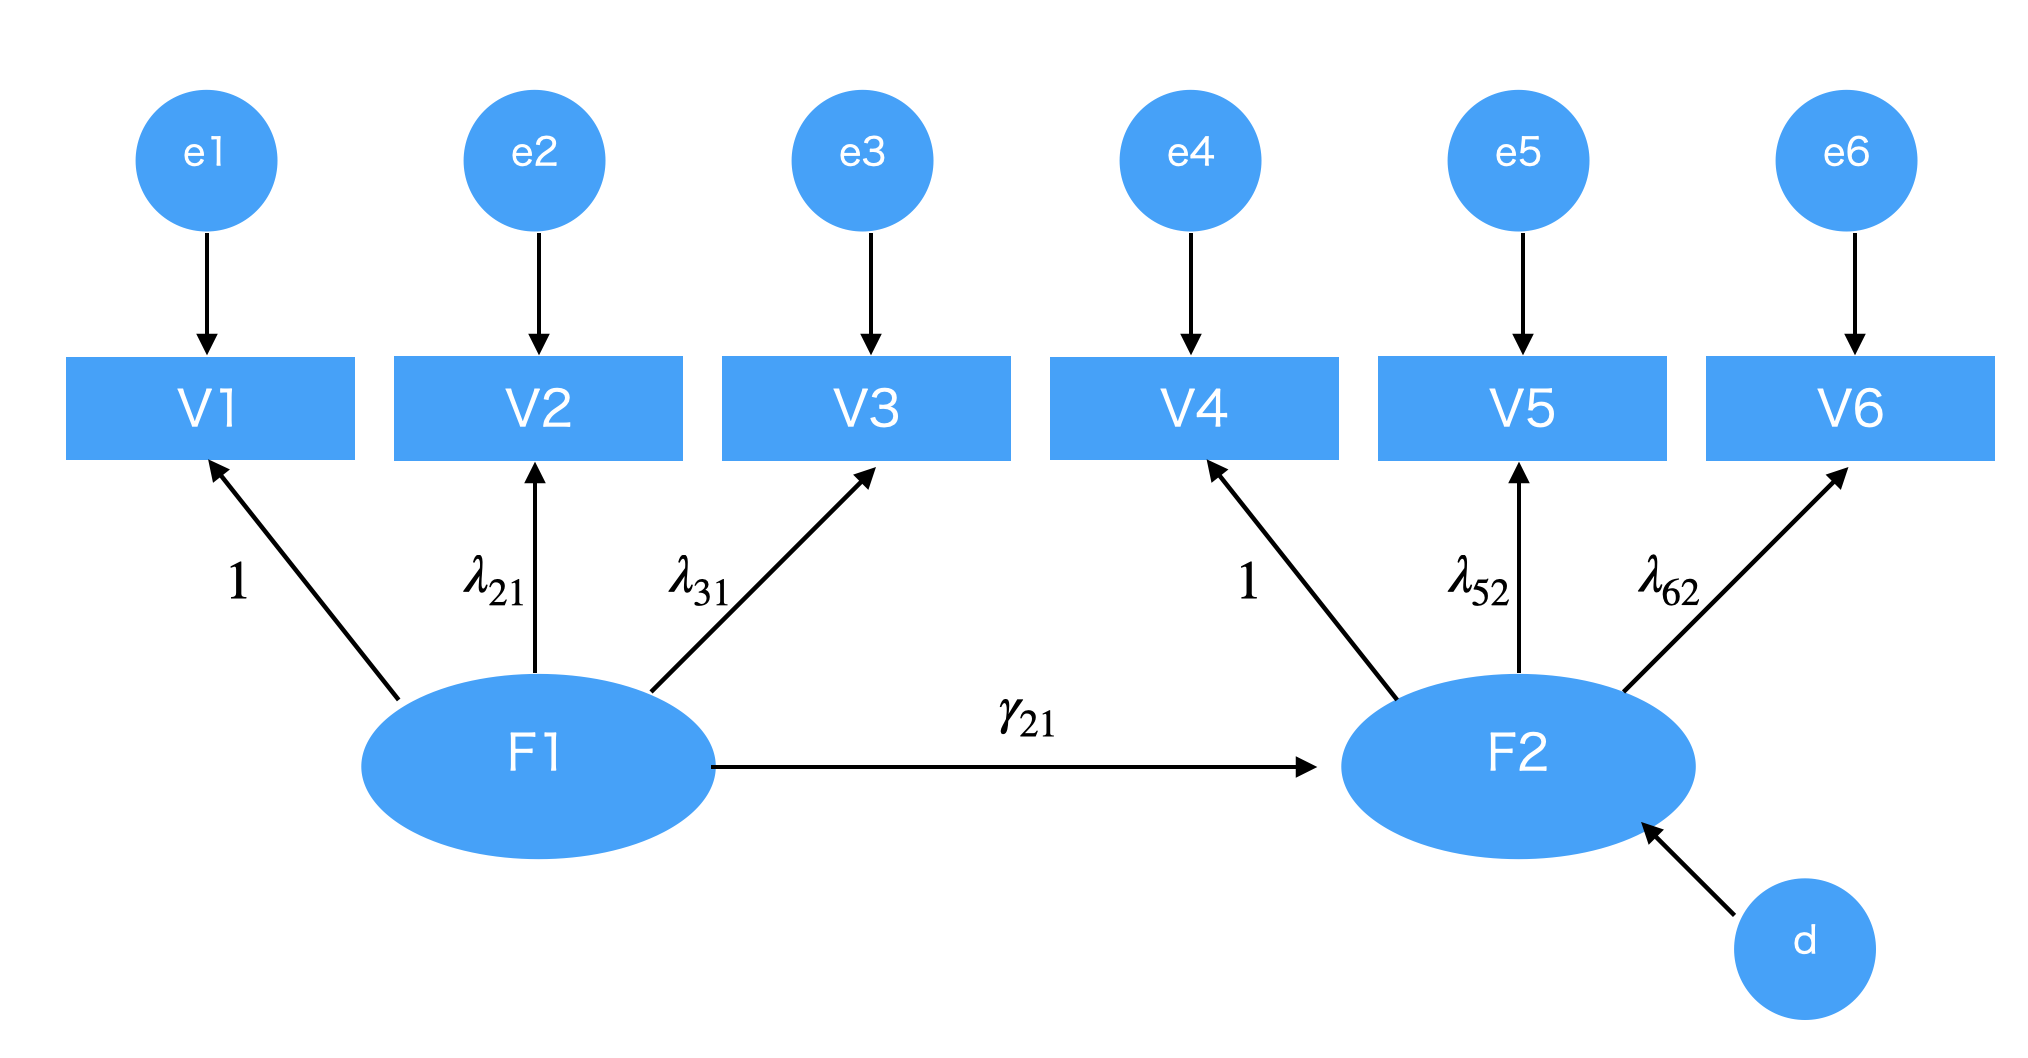
\includegraphics[width=0.8\linewidth,keepaspectratio]{../images/12_SEM/Slide12_05.png}
        \caption{構造方程式と測定方程式。記号の意味は後述}
        \label{fig::12_05}
    \end{center}
\end{figure}


% 図\ref{fig::12_05}には因子分析がふたつと，因子と因子の関係を矢印で結んだパスが描かれています。潜在変数の間に回帰分析を組み込んだようなものですね。イメージとしては，ある心理変数が別の心理変数に影響を与える(ex.外向性が抑うつ傾向に影響する，など)といったものを表しているわけです。心理学者は心理的変数がどう影響しあっているか，関係しあっているかをみていきたいわけですから，やりたいことは要するにこういう複合的なモデルによる検証だったのだ，と言っても過言ではないでしょう。このような分析も，SEMのおかげで簡単にできるようになりました。ここで観測変数から潜在変数を構成する箇所をとくに\keytermL{測定方程式}{そくていほうていしき}，潜在変数同志の因果関係などそれ以外の関係を表現する箇所を\keytermL{構造方程式}{こうぞうほうていしき}と呼んで区別することがありますが，\keytermL{構造方程式モデリング}{こうぞうほうていしきもでりんぐ}はその両者からなるモデル全体のこと，ということができるでしょう。
Figure \ref{fig::12_05} shows two factor analyses and paths that connect factors with arrows. It's like incorporating regression analysis between latent variables. As an image, it represents a psychological variable affecting another psychological variable (for example, extraversion affects depression tendency, etc.). Psychologists want to see how psychological variables influence and relate to each other, so what they want to do can arguably be said to be verification by such complex models. Thanks to SEM, such analyses can now be done easily. In this case, the parts where latent variables are constructed from observed variables are particularly referred to as \ keytermL {measurement equations}, and the parts that represent causal relationships and other relationships between latent variables are called \ keytermL {structural equations}. Although it is distinguished by calling, the overall model consisting of both can be said to be \ keytermL {structural equation modeling}.

% 構造方程式モデリングを使うと，調査などから得たデータ全体の見取り図を描いて分析できるのです。言い換えると，実際に調査を実施する前に，どの変数とどの変数がどのような関係にあるのか，という仮定を考えて調査票をデザインし，過不足なく測定してモデルを検証する，という\textbf{仮説検証型}の分析ができるのです。それまでの調査は，どういう変数がどういう関係になっているか細かくは分からないけれども，何か関係しそうだからまとめて調査項目にしておいて，因子分析や回帰分析を繰り返して，変数間の関係を\textbf{探索的に}研究するということがよく行われていました。もちろん今でも探索的研究はあるのですが，既存の尺度や先行研究がある場合はより具体的に調査を設計できるようになりました。
Using structural equation modeling, you can draw and analyze an overview of the entire data obtained from surveys. In other words, before actually conducting a survey, you can consider the assumption of how each variable relates to each other, design a survey form based on that assumption, and then verify the model by accurately measuring it. This allows for hypothetical verification analysis. Until then, although it was not known in detail how each variable was related, they were often included in survey items because they seemed to be related, and factor analysis and regression analysis were repeated to study the relationship between variables in an exploratory manner. Of course, exploratory research still exists today, but if there are existing scales and previous studies, we have been able to design surveys in a more concrete way.

% 因子分析も，因子数がわからないのでスクリープロットなどを描いて探し出し，因子と項目の関係がわからないのですべての因子がすべての項目に影響すると考えて分析する\keyterm{探索的因子分析}{たんさくてきいんしぶんせき}{Exploratory Factor Analysis,EFA}がかつては主流でしたが，今ではどの因子がどの項目で測定されるかを明確にパスダイアグラムで表現して分析する，\keyterm{検証的因子分析}{けんしょうてきいんしぶんせき}{Confirmatory Factor Analysis, CFA}が行われるようになってきています。
Factor analysis used to be mainly performed by exploratory factor analysis, where a scree plot or the like is drawn to search for the number of factors, and all factors are assumed to affect all items because the relationship between factors and items is unknown. Nowadays, however, confirmatory factor analysis, which clearly represents which factors are measured by which items in a path diagram and performs analysis, is becoming more common.



% \section{構造方程式モデルによる未知数の推定}
\section{Estimation of Unknowns using Structural Equation Modeling}
% \subsection{未知数は本当に推定できるのか}
\subsection{Can We Really Estimate the Unknowns?}
% さて，さまざまなモデルをパスダイアグラムで表現できる，ということがわかりましたが，「方程式」という言葉はどこからきているのでしょう？
So, we've learned that various models can be represented by path diagrams, but where does the word "equation" come from?
% 実は，統計モデルはパスダイアグラムでも表現できますが，同じことを方程式でも表現できます。
Actually, although statistical models can be represented by path diagrams, the same thing can be represented by equations as well.

% たとえば図\ref{fig::12_01}で表した回帰分析モデルは，次のような方程式で表せるのでした。
For example, the regression analysis model shown in Figure \ref{fig::12_01} could be expressed by the following equation.

\[ y = b_0 + b_1 x + e \]

図\ref{fig::12_02}に表した因子分析モデルも，同様に次のような方程式で表せるのでした(項目が3つの場合)。

\[ \left \{
	\begin{array}{rcl}
		x_1 & = & \lambda_1 f + e_1 \\
		x_2 & = & \lambda_2 f + e_2 \\
		x_3 & = & \lambda_3 f + e_3 \\
	\end{array}
	\right .
\]

% ここで$f$は因子得点，$\lambda_j$は因子負荷量，あるいはパス係数を表しています。
Here, $f$ represents the factor score, and $\lambda_j$ represents the factor load or the path coefficient.

% この因子分析モデルを例に，この方程式をどのように解くかをみていきましょう。そのために，いくつかの記号と特徴を確認します。まずベクトルの平均を関数$\bm{E}$で表すことにします。誤差の平均は0，という特徴は$\bm{E} \left[ \bm{e} \right] = \bm{0}$と表すことができます。因子得点も標準化されていると仮定しますので，$\bm{E} \left[ \bm{f}\right] = \bm{0}$ですね。つぎにベクトルの分散を関数$\bm{V}$で表すとします。データベクトル$\bm{x}$が平均0，あるいは平均偏差，あるいは標準化されていると考えると，$\bm{V} \left [ \bm{x} \right] =\bm{E} \left[ ( \bm{x} - \bm{E}\left[ \bm{x} \right] )^2 \right ] = \bm{E} \left [ \bm{xx'}\right]$は分散共分散行列$\bm{\Sigma}$だと考えることができます。また因子は標準化されているので$\bm{V}\left [ \bm{f} \right ] = 1$，誤差同士は相関しないものの，誤差には分散がありますので$\bm{V}\left[ \bm{e} \right]=\bm{E} \left[ \bm{ee'}\right] = \Psi$とします。ここで$\Psi$は対角に誤差分散が入った対角行列です。
Let's take a look at how to solve this equation using this factor analysis model as an example. For that purpose, let's confirm some symbols and features. First, let's denote the mean of vectors with the function $\bm{E}$. The characteristic that the mean of errors is 0 can be expressed as $\bm{E} \left[ \bm{e} \right] = \bm{0}$. Assume that the factor scores are also standardized, so $\bm{E} \left[ \bm{f}\right] = \bm{0}$. Next, we'll denote the variance of a vector with the function $\bm{V}$. If we consider the data vector $\bm{x}$ to be mean 0, or mean-deviated, or standardized, then $\bm{V} \left [ \bm{x} \right] =\bm{E} \left[ ( \bm{x} - \bm{E}\left[ \bm{x} \right] )^2 \right ] = \bm{E} \left [ \bm{xx'}\right]$ can be considered as the variance-covariance matrix $\bm{\Sigma}$. Also, since the factors are standardized, $\bm{V}\left [ \bm{f} \right ] = 1$, and although the errors do not correlate with each other, there is variance in the errors so $\bm{V}\left[ \bm{e} \right]=\bm{E} \left[ \bm{ee'}\right] = \Psi$. Here $\Psi$ is a diagonal matrix with error variances on the diagonal.

% さて，さきほどの3項目1因子モデルを行列で表現してみましょう。各要素を次のようにベクトルでまとめて表現します。
Now, let's represent the three-item, one-factor model we discussed earlier in matrix form. We'll group each element together as follows using vectors.
\[ \bm{x} = \begin{pmatrix} x_1\\x_2\\x_3 \end{pmatrix}, \bm{\Lambda} = \begin{pmatrix} \lambda_1\\ \lambda_2 \\ \lambda_3 \end{pmatrix}, \bm{e} = \begin{pmatrix} e_1 \\ e_2 \\ e_3 \end{pmatrix} \]
すると式は次のようにあっさり表現できます。
\[ \bm{x} = \bm{\Lambda} \bm{f} + \bm{e} \]
% ここからデータの分散共分散行列$\bm{\Sigma}$を考えてみましょう。
Let's consider the covariance matrix $\bm{\Sigma}$ of the data from here.

\begin{eqnarray*}
    \bm{V}\left[ \bm{x} \right] &=& \bm{E}\left[ \bm{xx'}\right]\\
    &=& \bm{E}\left[ (\bm{\Lambda f}+\bm{e}) (\bm{\Lambda f}+\bm{e})' \right] \\
    &=& \bm{E}\left[ (\bm{\Lambda f}+\bm{e}) (\bm{f \Lambda' }+\bm{e'}) \right] \\
    &=& \bm{E}\left[ \bm{ \Lambda f^2 \Lambda' + \Lambda f e'  + ef\Lambda ' + ee' } \right] \\
    &=& \bm{\Lambda \Lambda'} + \Psi \\
\end{eqnarray*}


% これをエレメントワイズで書き出すと次のようになります。
When written out element-wise, it becomes as follows.
\begin{eqnarray*}
    \begin{pmatrix} s_1^2 & s_1s_2 & s_1s_3 \\
                      & s_2^2  & s_2s_3 \\
                      &        & s_3^2\end{pmatrix}
    &=& \begin{pmatrix} \lambda_1\\ \lambda_2 \\ \lambda_3 \end{pmatrix}\begin{pmatrix} \lambda_1 & \lambda_2 & \lambda_3 \end{pmatrix} + \begin{pmatrix} \sigma_1^2 & & \\ & \sigma_2^2 & \\ & & \sigma_3^2 \end{pmatrix} \\
    &=& \begin{pmatrix} \lambda_11^2 + \sigma_1^2 & \lambda_1\lambda_2       & \lambda_1 \lambda_3      \\
                                          & \lambda_2^2 + \sigma_2^2 & \lambda_2 \lambda_3      \\
                                          &                          & \lambda_3^2 + \sigma_3^2\end{pmatrix}
\end{eqnarray*}


% この式の左辺はデータから計算された分散共分散行列，右辺はモデルから計算された分散共分散行列です。行列の下三角が消えているのは対称行列で同じ情報が入るからで，データからオリジナルに得られるのは3つの分散($s_1^2,s_2^2,s_3^2$)と3つの共分散($s_1s_2,s_1s_3,s_2s_3$)の情報になります。一方右辺での未知数はパス係数(因子負荷量)の$\lambda_1,\lambda_2,\lambda_3$と誤差分散$\sigma_1^2,\sigma_2^2,\sigma_3^2$ということになります。未知数の数と既知数の数が同じなので，この方程式は解けます。とくに，未知数と既知数の数が一致しているので，\keyterm{丁度識別}{ちょうどしきべつ}{just identification}，あるいは単に\keyterm{識別可能}{しきべつかのう}{identifiable}といいます。
The left side of this equation is the variance-covariance matrix calculated from the data, and the right side is the variance-covariance matrix calculated from the model. The reason why the lower triangle of the matrix disappears is because it is a symmetric matrix in which the same information is input. From the data, the original can yield the information of three variances ($s_1^2,s_2^2,s_3^2$) and three covariances ($s_1s_2,s_1s_3,s_2s_3$). On the other hand, the unknowns on the right side are the path coefficients (factor loads) of $\lambda_1,\lambda_2,\lambda_3$ and the error variances $\sigma_1^2,\sigma_2^2,\sigma_3^2$. Since the number of unknowns and the number of knowns are the same, this equation can be solved. In particular, since the number of unknowns and knowns is the same, it is referred to as "just identification" or simply "identifiable".

% 分散共分散行列で提供される情報の増え方に比べて，モデルの未知数の増え方は小さいので，一般的なSEMのモデルのほとんどは\keytermL{過剰識別}{かじょうしきべつ}になります。つまりいくつかの答えがあり得る，ということになるので，その時は尤度が最も高くなるように，といった基準を加えて答えを一意に定めます。逆に未知数の方が多い場合\keytermL{識別不可能}{しきべつふかのう}(解が求められない)ということになり，その場合はどこかのパラメータを値として入れてやる(\keytermL{制約}{せいやく}をかける，といいます)必要があります。
The increase in the number of unknowns in the model is smaller than the increase in information provided by the variance-covariance matrix, so most of the models in the general SEM become over-identified. This means that there could be multiple answers, so at that time we add criteria to specify the answer uniquely, such as maximizing the likelihood. On the other hand, if there are more unknowns, it becomes unidentifiable (the solution cannot be determined), and in that case, it is necessary to input some parameters as values (this is called imposing constraints).

% \subsection{複雑なモデルの場合}
\subsection{In the Case of Complex Models}

% では次に，図\ref{fig::12_05}のような複雑なモデルでも方程式で表せることを示しましょう。
Let's then demonstrate that even complex models like Fig.12_05 can be represented by equations.

% ここで図\ref{fig::12_05}の係数について説明します。ギリシア文字$\lambda$や$\gamma$がパス係数を表しています。パス係数の添字は，被説明変数の変数番号$j$と，説明変数の変数番号$k$をつかって$\lambda_{jk}$のようにかき，これで$k \to j$の影響力の大きさを表していると思ってください。測定方程式の係数を$\lambda$で，構造方程式の係数を$\gamma$で表現しました。また$\lambda_{11},\lambda_{42}$になるべきところが$1$になっていますが，これは「潜在変数から出るパスのうち，1つは必ず$1$にしないと推定できない」という数学的特徴があるからです。決まりごとだと思ってください。
Here, we will explain the coefficients in Figure \ref{fig::12_05}. Greek letters $\lambda$ and $\gamma$ represent path coefficients. The subscript of the path coefficient uses the variable number $j$ of the dependent variable and the variable number $k$ of the explanatory variable, written as $\lambda_{jk}$. Think of this as representing the magnitude of the influence from $k \to j$. The coefficient of the measurement equation is represented by $\lambda$, and the coefficient of the structural equation is represented by $\gamma$. Although where it should be $\lambda_{11},\lambda_{42}$, it has become $1$, this is due to a mathematical feature that "one of the paths from the latent variables cannot be estimated unless it is always set to $1$". Please think of it as a rule.

% それを踏まえて，モデルの方程式を書くと，次のようになります。
Considering that, when we write the equation of the model, it becomes as follows.
\[ \left \{
	\begin{array}{rcl}
		V_1 & = & f_1 + e_1             \\
		V_2 & = & \lambda_{21}f_1 + e_2 \\
		V_3 & = & \lambda_{31}f_1 + e_3 \\
		V_4 & = & f_2 + e_4             \\
		V_5 & = & \lambda_{52}f_2 + e_5 \\
		V_6 & = & \lambda_{62}f_2 + e_6 \\
		f_2 & = & \gamma_{21}f_1 + d
	\end{array}
	\right .
\]
% ややこしいだけで，書けるのは書けましたね！そして当然，これは行列表現した方が楽ではないか，というアイデアが浮かぶと思います。その通りで，エレメントワイズにまずは書いてみましょう。
It was a bit complicated, but you were able to write it, right? And naturally, I think you'll come up with the idea that it would be easier to represent this in matrix form. That's right, let's first write it out element-wise.

\[
	\begin{pmatrix} V_1 \\ V_2 \\ V_3 \\ V_4 \\ V_5 \\ V_6 \\ f_2 \\f_1 \end{pmatrix} =
	\begin{pmatrix} 0 & 0 & 0 & 0 & 0 & 0 & 0            & 1            \\
                0 & 0 & 0 & 0 & 0 & 0 & 0            & \lambda_{21} \\
                0 & 0 & 0 & 0 & 0 & 0 & 0            & \lambda_{31} \\
                0 & 0 & 0 & 0 & 0 & 0 & 1            & 0            \\
                0 & 0 & 0 & 0 & 0 & 0 & \lambda_{52} & 0            \\
                0 & 0 & 0 & 0 & 0 & 0 & \lambda_{62} & 0            \\
                0 & 0 & 0 & 0 & 0 & 0 & 0            & \gamma_{21}  \\
                0 & 0 & 0 & 0 & 0 & 0 & 0            & 0\end{pmatrix}
	\begin{pmatrix} V_1 \\ V_2 \\ V_3 \\ V_4 \\ V_5 \\ V_6 \\ f_2 \\f_1 \end{pmatrix} +
	\begin{pmatrix} e_1 \\ e_2 \\ e_3 \\ e_4 \\ e_5 \\ e_6 \\ d \\f_1 \end{pmatrix}
\]

% 左辺のベクトルの最後に$f_1$が入っているところがポイントで，これは方程式的には$f_1=f_1$というだけの式なのですが，これを入れたおかげで全体を整合的に表現できましたね。
The point here is that the vector on the left-hand side ends with $f_1$. In terms of the equation, this is just an expression saying $f_1=f_1$. Thanks to including this, we were able to express the whole thing in a coherent way.
% この左辺のベクトルを$\bm{v}$として，式全体を$\bm{v} = \bm{Gv}+\bm{e}$と考えてみましょう。すると次のように展開できます。
Let's consider the vector on the left side as $\bm{v}$, and the whole equation as $\bm{v} = \bm{Gv}+\bm{e}$. Then, it can be developed as follows.

\begin{eqnarray*}
    \bm{v} &=& \bm{Gv}+\bm{e}\\
    \bm{v}-\bm{Gv} &=& \bm{e}\\
    (\bm{I}-\bm{G})\bm{v} &=& \bm{e}\\
    (\bm{I}-\bm{G})^{-1}(\bm{I}-\bm{G})\bm{v} &=& (\bm{I}-\bm{G})^{-1}\bm{e}\\
\end{eqnarray*}

% ここで$\bm{P} = (\bm{I}-\bm{G})$とすると，
If we set $\bm{P} = (\bm{I}-\bm{G})$ here,
\[ \bm{v} = \bm{P}^{-1}\bm{e} \]
ということになります。これをエレメントワイズで書くと次のようになります。
\[
	\begin{pmatrix} V_1 \\ V_2 \\ V_3 \\ V_4 \\ V_5 \\ V_6 \\ f_2 \\f_1 \end{pmatrix} =
	\begin{pmatrix} 1 & 0 & 0 & 0 & 0 & 0 & 0             & -1            \\
                0 & 1 & 0 & 0 & 0 & 0 & 0             & -\lambda_{21} \\
                0 & 0 & 1 & 0 & 0 & 0 & 0             & -\lambda_{31} \\
                0 & 0 & 0 & 1 & 0 & 0 & -1            & 0             \\
                0 & 0 & 0 & 0 & 1 & 0 & -\lambda_{52} & 0             \\
                0 & 0 & 0 & 0 & 0 & 1 & -\lambda_{62} & 0             \\
                0 & 0 & 0 & 0 & 0 & 0 & 1             & -\gamma_{21}  \\
                0 & 0 & 0 & 0 & 0 & 0 & 0             & 1\end{pmatrix}
	\begin{pmatrix} e_1 \\ e_2 \\ e_3 \\ e_4 \\ e_5 \\ e_6 \\ d \\f_1 \end{pmatrix}
\]

% さて，変数からなるベクトル$\bm{v}$ではありますが，観測変数は$V_1$から$V_6$までしかありませんから，そこだけを取り出す行列$\bm{F}=\{ \bm{I},\bm{O} \}$を考えます。ここでは次のような行列です。
Well, we have a vector $\bm{v}$ consisting of variables, but we only have observation variables from $V_1$ to $V_6$, so we consider a matrix $\bm{F}=\{ \bm{I},\bm{O} \}$ that extracts only those. Here is what the matrix looks like.
\[
	\bm{F} =
	\begin{pmatrix} 1 & 0 & 0 & 0 & 0 & 0 & 0 & 0 \\
                0 & 1 & 0 & 0 & 0 & 0 & 0 & 0 \\
                0 & 0 & 1 & 0 & 0 & 0 & 0 & 0 \\
                0 & 0 & 0 & 1 & 0 & 0 & 0 & 0 \\
                0 & 0 & 0 & 0 & 1 & 0 & 0 & 0 \\
                0 & 0 & 0 & 0 & 0 & 1 & 0 & 0\end{pmatrix}
\]
% これを使って，次のように関係を書き直すことができます。
With this, you can rewrite the relationship as follows.

\[
	\bm{g} = \begin{pmatrix}  V_1 \\ V_2 \\ V_3 \\ V_4 \\ V_5 \\ V_6 \end{pmatrix} = \bm{FP^{-1}e}
\]
% さて，ではデータだけのベクトル$\bm{g}$から分散共分散行列を構成するとしましょう。データベクトル$\bm{g}$は平均が0だと仮定します\footnote{ずいぶんと勝手な仮定だな，と思うかもしれませんが，分析の元になる変数ベクトルを標準化したと思っていただければそれほどおかしなことでもない，と考えてもらっても構いません。あるいは単に変数ごとの平均をとった平均偏差ベクトルを作って，それをデータだとしたと考えてください。}。そうすると分散共分散行列$\bm{\Sigma}$は次のようになります。
Now, let's construct a variance-covariance matrix from the vector $\bm{g}$ of data alone. We assume that the data vector $\bm{g}$ has a mean of 0\footnote{You may think that's a rather arbitrary assumption, but you might not think it's so strange if you think of it as standardizing the variable vector that forms the basis for the analysis. Alternatively, you can think of it as creating a mean deviation vector by averaging each variable and considering that as the data.}. In this case, the variance-covariance matrix $\bm{\Sigma}$ will be as follows.

\begin{eqnarray*}
	\bm{\Sigma} &=& \bm{gg'}  \\
	& = & \bm{ F P^{-1} e ( F P^{-1} e) '} \\
	& = & \bm{ FP^{-1} ee' P^{-1'} F' }
\end{eqnarray*}


% ここで式の中にある$\bm{ee'}$は誤差などの未知数で作った分散共分散行列になっています。誤差は他の変数との共分散がないと考えられるので，これは結局対角行列です。
The $\bm{ee'}$ in the formula here represents a covariance matrix created from unknowns such as errors. Since it is considered that the error has no covariance with other variables, this is ultimately a diagonal matrix.
\[
	\bm{ee'}= \begin{pmatrix}  V(e_1) &        &        &        &        &  &        &      &        \\
                        & V(e_2) &        &        &        &  &        &      &        \\
                        &        & V(e_3) &        &        &  &        &      &        \\
                        &        &        & V(e_4) &        &  &        &      &        \\
                        &        &        &        & V(e_5) &  &        &      &        \\
                        &        &        &        &        &  & V(e_6) &      &        \\
                        &        &        &        &        &  &        & V(d) &        \\
                        &        &        &        &        &  &        &      & V(f_1)\end{pmatrix}
\]

% さあややこしい話はここまでにして，何を考えていたのかをもう一度考えてみましょう。
Let's end the complicated discussion here, and try to rethink what we were considering once again.

% この式の左辺は$\bm{\Sigma}$，すなわちデータからできる分散共分散行列であり，具体的に数字の計算のできるデータセットです。この式の右辺は$\bm{ FP^{-1} ee' P^{-1'} F' } $であり，係数と潜在変数の分散からなる方程式です。左辺にデータ，右辺にモデルで表した分散共分散行列があり，これがイコールで結びついているのですから，この連立方程式を解けば，係数を求めることができます。
The left side of this equation is $\bm{\Sigma}$, which is the variance-covariance matrix that can be created from the data, and is a specific data set that can be calculated numerically. The right side of the equation is $\bm{ FP^{-1} ee' P^{-1'} F' } $, which consists of coefficients and the variance of latent variables. There is a variance-covariance matrix represented by the model on the right side and data on the left side, and since these are connected by an equal sign, solving this simultaneous equation allows you to find the coefficients.

% そりゃその計算はとても面倒なことになると思われますが，そこは機械がやってくれるのだ，と割り切ればいいでしょう。モデルがデータに最も合うように，未知数を決めていく方法は，\keytermL{最小二乗法}{さいしょうにじょうほう}や\keytermL{最尤法}{さいゆうほう}など，今まで学んできた手法を使えばよいのです！
While it seems like these calculations could become very tedious, it's fine to just settle on the idea that the machine will take care of it for us. The method of determining unknowns such that the model best fits the data, such as the least squares method or the maximum likelihood method, is one we've been learning so far!

% こうして自由なモデリング技術とその解法を私たちは手に入れることができました。構造方程式モデリングとは，変数間関係を細かく作り込んでいき，分散共分散行列の隅々まで考え尽くす究極のモデル，と意味が伝わったでしょうか。
In this way, we were able to acquire free modeling techniques and their solutions. Structural equation modeling is the ultimate model that meticulously constructs relationships between variables and thoroughly considers every corner of the variance-covariance matrix. I hope the meaning has been conveyed.

% \section{適合度によるモデルの評価}
\section{Evaluation of Model by Suitability}

% データ行列とモデル行列をイコールで結んだ方程式を解くことが，未知数を求める根本的な原理であるということがわかりました。
I understood that solving the equation connecting the data matrix and the model matrix with an equal sign is the fundamental principle of obtaining unknown numbers.
% 方程式が多く未知数が少ない場合，値が一意に定まらな苦なってしまいます\footnote{たとえば$x+5=8$と$x-3=9$という連立方程式があればどうでしょうか。未知数は1つ，式は2つなのでどちらが正解なのかわかりません！}。これはパラメータに\keyterm{自由度}{じゆうど}{degrees of freedom}がある，ということもできます。そのような場合は別の基準をつかって最も良いと考えられる数字を推定値として用いることになります。
When there are more equations than unknowns, the value does not uniquely determine itself\footnote{For example, what if there are simultaneous equations like $x+5=8$ and $x-3=9$? There is one unknown and two expressions, so we don't know which one is correct!}. This can also be referred to as having "degrees of freedom" in the parameters. In such situations, we use a different standard to consider the best number as the estimated value.

% さてなんとかモデルをデータに当てはめることができたとして，それがどの程度一致しているか，ということは別次元で評価しなければなりません。それが\keyterm{適合度}{てきごうど}{fit index}です。SEMの文脈では複数の適合度が考えられており，それらを総合的に評価するというやり方がとられています。ここでは複数の適合度指標をご紹介しておきます\footnote{以下の記述は\citet{Kosugi2014Mplus}をもとに加筆修正したものです。}。
Assuming we have somehow been able to fit the model to the data, we need to evaluate how well it fits in a separate dimension. That's where the \keyterm{fit index} comes in. In the context of SEM, several fit indices are considered, and an approach of evaluating them comprehensively is undertaken. Here, we introduce multiple fit indices\footnote{The description below is modified based on \citet {Kosugi2014Mplus}.}.

% \paragraph{GFI・AGFI} \keyterm{GFI}{GFI}{Goodness of Fit Index}や\keyterm{AGFI}{AGFI}{Adjusted GFI}は，0から1までの値を取る適合度指標で，因果モデルがデータの何\%を説明したかの指標になります。1に近いほど良いモデルで，GFIで0.95,AGFIで0.90以上の数字であると良い適合と判断されます。
\paragraph{GFI・AGFI} The \keyterm{GFI}{GFI}{Goodness of Fit Index} and \keyterm{AGFI}{AGFI}{Adjusted GFI} are fit indices that take values from 0 to 1, indicating what percentage of the data is explained by the causal model. The closer the value is to 1, the better the model. It is judged that numbers that are 0.95 for GFI and 0.90 or higher for AGFI show good fit.

% \paragraph{情報量規準}
I'm sorry but you haven't provided any Japanese text for me to translate. Please provide some content for translation.
% \keyterm{情報量規準}{じょうほうりょうきじゅん}{Information Criteria}とは，一般的な統計モデルを評価するための指標で，\keyterm{AIC}{AIC}{Akaike's Infromation Criterion}や\keyterm{BIC}{BIC}{Bayesian I.C.}などがそれにあたります。これは今検証しているモデルが，データによくフィットする「本当の」モデルからどの程度離れているかを示す指標です。本当のモデル，というのは分かり得ませんから，複数のモデルA,B,Cを同じデータに当てはめたとき，AICやBICが相対的に小さいものが，より良く適合していると判断します。相対的な指標ですから，違う変数を扱うモデル間の比較はできないことに注意が必要です。
"Information Criteria" is a metric for evaluating general statistical models, which includes "AIC (Akaike's Information Criterion)" and "BIC (Bayesian Information Criterion)". This is a metric that indicates how far the model being tested is from the "true" model that fits well with the data. The "true" model is unknown, so when multiple models A, B, C are applied to the same data, the one with the relatively smaller AIC or BIC is judged to be better fitting. It is a relative metric, so it is important to note that comparison between models dealing with different variables is not possible.
\paragraph{RMSEA}
% モデルがデータとどの程度乖離しているか、を直接表現した指標が\keyterm{RMSEA}{RMSEA}{Root Mean Square Error of Approximation}です。近似した誤差に対する平方平均平方根，ということですね。一般に0.05より小さければ，そのモデルは当てはまりがよく，0.1以上であれば当てはまりが悪いと判断します。
The metric that directly represents how much the model deviates from the data is the \keyterm{RMSEA}{RMSEA}{Root Mean Square Error of Approximation}. It refers to the root mean square of the approximation error. Generally, if it's less than 0.05, the model fits well, and if it's more than 0.1, the model is considered a poor fit.
\paragraph{CFI/TLI}
% \keyterm{CFI}{CFI}{Comparatative Fit Index}や\keyterm{TLI}{TLI}{Tucker-Lewis Index}は，観測変数間にまったく相関がないという非現実的なモデル（独立モデルという）に比べて，当該のモデルがどの程度よいものかを指標化したものです。いずれも1.0に近ければ近いほど良いモデルとされています。一般にこの数値が0.9以上になることを目指してモデルを改訂していきます。
The Comparative Fit Index (CFI) and the Tucker-Lewis Index (TLI) are indicators that measure how good a model is compared to an unrealistic model (called the independent model) that assumes there is absolutely no correlation between observed variables. The closer either index is to 1.0, the better the model is considered. Generally, we aim to revise the model so that this value is above 0.9.
\paragraph{SRMR}
% \keyterm{SRMR}{SRMR}{Standardized Root Mean square Residual}は標準化された残差平方平均平方根を表します。これはモデルで説明できなかったものがどれほどあったか，を表しますので，0に近ければ近いほど当てはまりの良いことを表します。
"SRMR (Standardized Root Mean Square Residual) represents the standardized root mean square residual. This expresses how much of what could not be explained by the model remains, so the closer it is to zero, the better the fit."
% \paragraph{修正指数}
Sure, I would need the Japanese text to proceed with the translation.
% 最後に，\keyterm{修正指数}{しゅうせいしすう}{modification index}を紹介しておきます。
Finally, let me introduce the \keyterm{modification index}.
% 上で述べたように，検証しようとした統計モデルがどの程度当てはまっているか，ということを数値化できるようになったわけですが，常に最初にたてた仮説モデルが最適である，ということは滅多にありません。データから仮説の訂正を余儀なくされることがある，あるいはもっと良くなったり新しい発見があったりすることが，統計モデリングの醍醐味でもあります。修正指数は，どこをどう改良すれば指標がよくなりますよ，というヒントを与えてくれるものです。もっとも，適合度を上げることだけが目的なのではないことに注意してください。適合度を上げるために，意味のわからないモデルを作り上げたところで，モデルの意味がないのですから。
As mentioned above, we have now been able to quantify how well the statistical model we tried to verify fits. However, it is rarely the case that the initial hypothesis model we set up is optimal. There may be times when we have to revise our hypothesis from the data, or there may be times when we find something better or discover something new. This is also one of the attractions of statistical modeling. The correction index gives us hints on how and where to improve our indicators. However, please be aware that the purpose is not just to increase the fit. Even if you create a meaningless model to increase the fit, it is meaningless because the model doesn't make sense.



% 構造方程式モデリングは，非常に複雑な方程式を解いているんだな，ということは理解していただけたかと思います。
I believe you have understood that structural equation modeling is solving very complex equations.
% 次回はそんな複雑なモデルでも，Rで簡単に分析できるよということを，演習を交えて理解していきましょう。
Next time, let's understand, through exercises, that even such complex models can be easily analyzed in R.
% \section{課題}
\section{Assignment}
% 2項目1因子モデルの方程式，およびそれを行列形式で表したものを書きましょう。
Let's write the equation of the two-item one-factor model, and its matrix form.

% また行列の要素で書いた場合，既知数と未知数はどちらが多くなるでしょうか。言い換えれば，このモデルは識別できるでしょうか。式を展開して確認してください。
When writing in terms of matrix elements, which will be more, the known or the unknowns? In other words, is this model identifiable? Please expand the formula and check.

\end{document}
